    % This file is part of nrf_seminar.

    % nrf_seminar is free software: you can redistribute it and/or modify
    % it under the terms of the GNU General Public License as published by
    % the Free Software Foundation, either version 3 of the License, or
    % (at your option) any later version.

    % nrf_seminar is distributed in the hope that it will be useful,
    % but WITHOUT ANY WARRANTY; without even the implied warranty of
    % MERCHANTABILITY or FITNESS FOR A PARTICULAR PURPOSE.  See the
    % GNU General Public License for more details.

    % You should have received a copy of the GNU General Public License
    % along with nrf_seminar.  If not, see <https://www.gnu.org/licenses/>.

\begin{textblock}{8.}(0., -4.)
    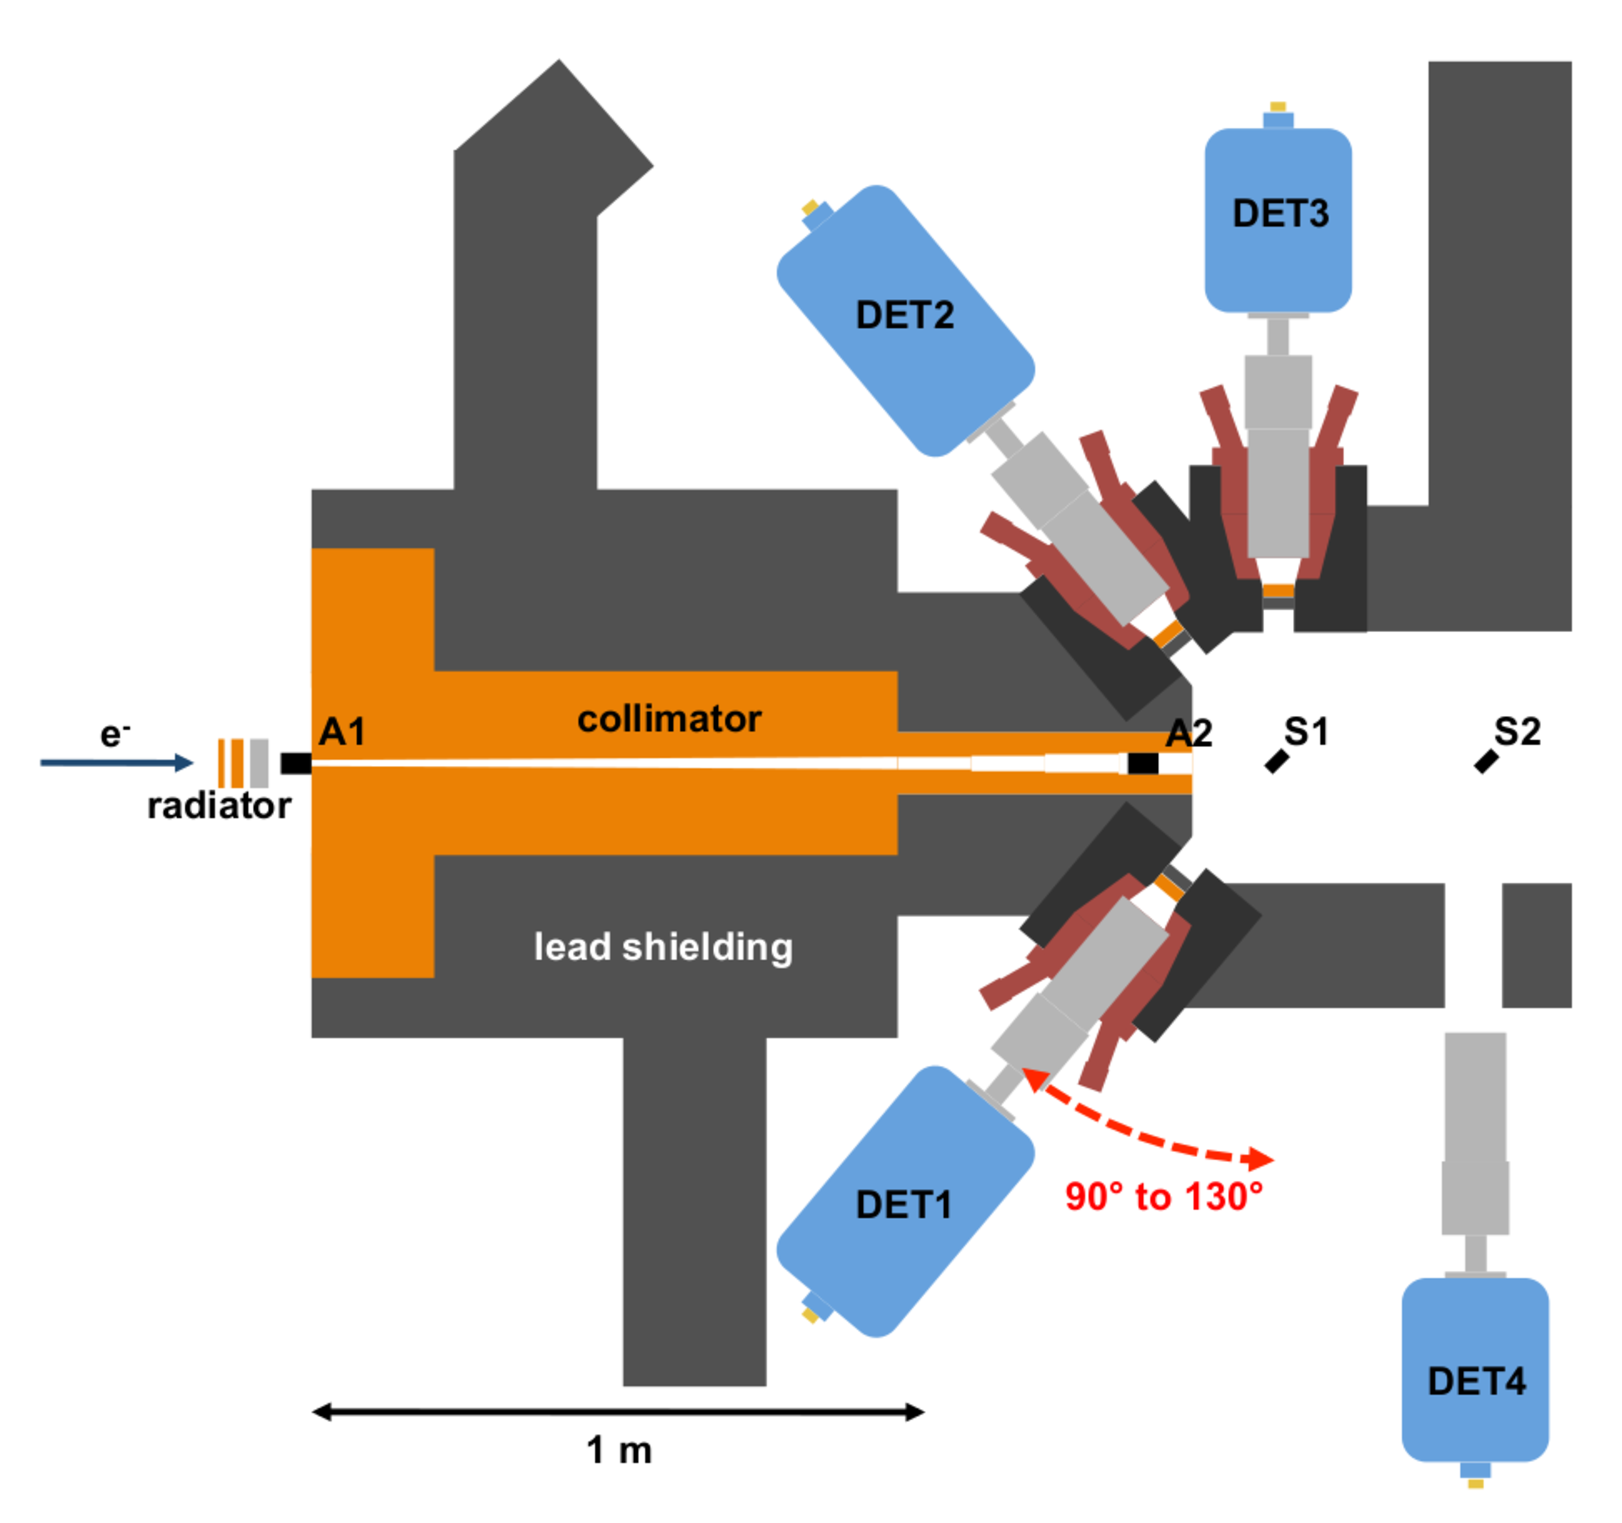
\includegraphics[width=\textwidth]{figures/dhips.pdf}
\end{textblock}

\begin{textblock}{6.}(9., -5.)
    \begin{itemize}
        \item Hayward et al. (1957)
        \item Continuous spectrum of photons up to the maximum electron energy
    \end{itemize}
\end{textblock}

\def \SPECTRUMX {9.}
\def \SPECTRUMY {0.}

\begin{textblock}{6.}(\SPECTRUMX, \SPECTRUMY)
    \visible<2>{
        \includegraphics[width=\textwidth]{figures/python/bremsstrahlung_linear.pdf}
    }
\end{textblock}

\begin{textblock}{6.}(\SPECTRUMX, \SPECTRUMY)
    \visible<3>{
        \includegraphics[width=\textwidth]{figures/python/bremsstrahlung_logarithmic.pdf}
    }
\end{textblock}